\documentclass{beamer}
\usepackage[utf8]{inputenc}
\usepackage[T1]{fontenc}
\usepackage[spanish,es-tabla]{babel}
\usepackage{booktabs,graphicx,tikz}
\usetikzlibrary{arrows.meta,positioning}
\usepackage{tesis_beamer}

\graphicspath{{../tesis/imagenes/}}

% Notación compartida con la tesis
\newcommand{\JLoss}{\mathrm{JLoss}}
\newcommand{\GaR}{\mathrm{GaR}}
\newcommand{\Spread}{\mathrm{spread}}

\author{Mauricio Valenzuela Corvalán}
\institute[Universidad de Chile]{Departamento de Ingeniería Civil Industrial\\
\small Magíster en Economía Aplicada · Universidad de Chile}
\title[Fragilidad bancaria y riesgo de cola]{Fragilidad bancaria sistémica y riesgo de cola del crecimiento}
\subtitle{Determinantes del \textit{spread} soberano en economías emergentes}
\date{\today}

\setbeamertemplate{navigation symbols}{}

\begin{document}

\begin{frame}
\titlepage
\vspace{-8pt}
\centering
\footnotesize Profesor guía: Juan Francisco Martínez Sepúlveda \quad\quad
Profesor coguía: Ronald Fischer
\end{frame}

\begin{frame}{Tabla de contenidos}
\tableofcontents[sectionstyle=show,subsectionstyle=show/shaded/hide]
\end{frame}

\section{Motivación y objetivos}

\begin{frame}{El mecanismo: un \textit{doom loop} banca--soberano}
\begin{center}
\resizebox{0.62\textwidth}{!}{%
\begin{tikzpicture}[
  node distance=7mm and 0mm,
  box/.style={draw, thick, rounded corners, align=center, fill=gray!7,
              minimum width=6.6cm, minimum height=1.0cm, font=\small},
  boxhi/.style={box, draw=tesisblue, fill=tesisblue!8, line width=1pt},
  lbl/.style={font=\scriptsize\itshape, align=left, text width=3.2cm}
]
\node[box]              (gar)    {Riesgo de cola del crecimiento ($\GaR$)};
\node[box, below=of gar]   (estr)   {Estructura y conducta del sistema bancario};
\node[boxhi, below=of estr] (jloss)  {Fragilidad sistémica ($\JLoss$)};
\node[boxhi, below=of jloss] (spread) {\textit{Spread} soberano (EMBI)};
\draw[-{Latex[length=2.2mm]}] (gar)   -- (estr)   node[midway, right, lbl] {modula el impacto};
\draw[-{Latex[length=2.2mm]}] (estr)  -- (jloss)  node[midway, right, lbl] {riesgo fiscal implícito};
\draw[-{Latex[length=2.2mm]}, tesisblue, line width=0.9pt] (jloss) -- (spread) node[midway, right, lbl, tesisblue] {\textbf{estimado en esta tesis}};
\draw[-{Latex[length=2.2mm]}, dashed, gray!50!black]
  (spread.west) to[bend left=45] node[midway, left, lbl, text width=2.6cm] {retroalimentación\\(costo de fondeo)} (estr.west);
\end{tikzpicture}%
}
\end{center}
\vspace{2pt}
\small
\begin{itemize}
\item La fragilidad bancaria y el riesgo de cola del crecimiento no son aditivos: se \textbf{complementan} en su transmisión al riesgo soberano.
\item Pregunta: ¿amplifica su coincidencia el spread soberano por encima de la suma de sus efectos individuales?
\end{itemize}
\end{frame}

\begin{frame}{Objetivos (Informe de Taller de Tesis I, dic. 2025)}
\textbf{Objetivo general.} Evaluar empíricamente el impacto conjunto, estructural y no lineal de la fragilidad del sistema bancario ($\JLoss$) y el riesgo de cola del crecimiento ($\GaR$) sobre el \textit{spread} de crédito soberano en economías emergentes.
\vspace{6pt}

\textbf{Hipótesis central.} El mercado penaliza de forma no lineal la coexistencia de fragilidad bancaria y vulnerabilidad macroeconómica.
\vspace{6pt}

\textbf{Muestra piloto (4 países, 2008--2022):}
\begin{itemize}
\item \textit{Pooled} sin efectos fijos: interacción $JLoss\times GaR$ \textbf{no significativa} ($p=0{,}641$).
\item Panel con efectos fijos país+tiempo: interacción \textbf{altamente significativa} ($p<0{,}0001$) --- ``la evidencia central de la tesis''.
\end{itemize}
\vspace{4pt}
\textit{Esta tesis pone ese hallazgo a prueba a escala global, con un motor de datos propio.}
\end{frame}

\section{Datos y metodología}

\begin{frame}{Un solo panel, tres piezas}
\begin{columns}[T]
\column{0.33\textwidth}
\textbf{$\JLoss$} — fragilidad bancaria\\[2pt]
\footnotesize Punto de silla de PD tipo Merton--KMV, 113 bancos, protocolo único de extracción Bloomberg
\column{0.33\textwidth}
\textbf{$\GaR$} — riesgo de cola\\[2pt]
\footnotesize Regresión cuantílica de panel (cuantil 5\%), marco \textit{vulnerable growth}, pseudo--tiempo real
\column{0.33\textwidth}
\textbf{EMBI} — \textit{spread} soberano\\[2pt]
\footnotesize J.P. Morgan, EMBI Global Diversified; CDS 5A como robustez
\end{columns}
\vspace{6pt}
\begin{block}{Especificación de referencia}
\centering
$\Spread_{i,t} = \alpha_i + \gamma_t + \beta_1 \JLoss_{i,t} + \beta_2^{D} D_{i,t} + \beta_3(\JLoss\times D)_{i,t} + \omega'X_{i,t} + \epsilon_{i,t}$
\end{block}
\footnotesize $D\equiv-\GaR$ (mayor $D$ = cola más adversa) $\Rightarrow$ $\beta_3>0$ señala amplificación. FE país+tiempo, errores Driscoll--Kraay.
\end{frame}

\begin{frame}{El panel: 13 países, 2004Q1--2026Q1}
\begin{center}
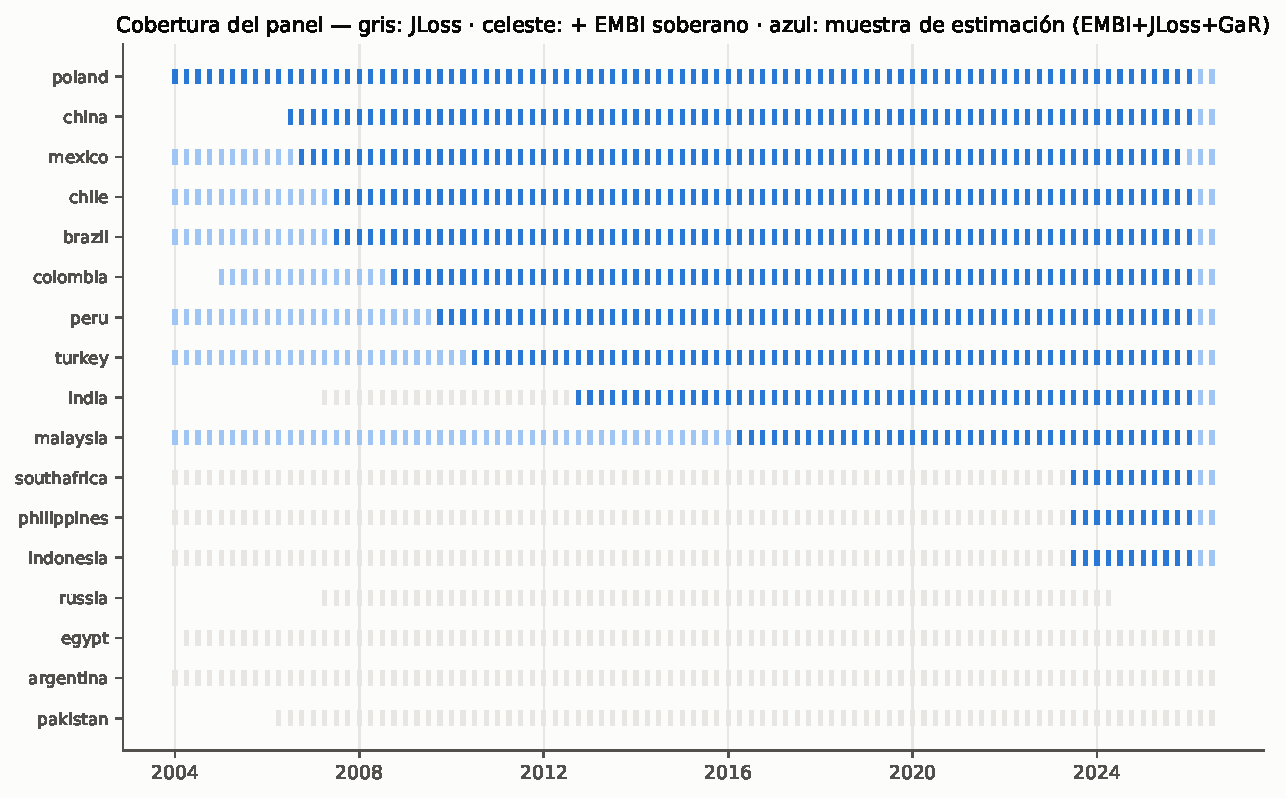
\includegraphics[width=0.92\textwidth]{fig_cobertura.pdf}
\end{center}
\footnotesize $N=721$ (sin controles) / $N=614$ (con 6 controles domésticos). Corea del Sur, Bulgaria y Hungría excluidos por $\JLoss$ no válido a nivel país.
\end{frame}

\begin{frame}{Por qué interactuar: las tres series co-mueven}
\begin{center}

\includegraphics[width=0.85\textwidth]{fig_comovimiento.pdf}
\end{center}
\footnotesize $D=-\GaR$, $\JLoss$ y EMBI, estandarizados y agregados por mediana transversal. Se mueven marcadamente juntas en 2008--09 y 2020 --- la motivación directa del término $\JLoss\times D$.
\end{frame}

\section{Resultados}

\begin{frame}{Los canales de nivel se sostienen (H1, H2)}
\begin{itemize}
\item $\hat\beta_1 (\JLoss) = +2{,}8$ pb por unidad ($t=2{,}7$) --- significativo al 1\% en las 12 especificaciones de la batería principal.
\item Coef. de $D=-\GaR$ $= +4{,}3$ pb ($t=2{,}3$) --- mayor riesgo de cola eleva el spread.
\item Respaldo dinámico de H1: proyecciones locales, pico $+4{,}6$ pb ($t=2{,}9$), un trimestre después del choque.
\end{itemize}
\vspace{8pt}
\begin{alertblock}{Pero la interacción, sobre la muestra completa...}
$\hat\beta_3=+0{,}16$ ($p=0{,}26$ DK; $p=0{,}14$ \textit{wild cluster bootstrap}) --- \textbf{no significativa}.
\end{alertblock}
\end{frame}

\begin{frame}{Eso es un promedio de regímenes}
La no significancia de la muestra completa esconde dos dimensiones donde la complementariedad \textbf{sí} aparece:
\vspace{6pt}
\begin{block}{Transversal --- núcleo de financiamiento externo}
$\hat\beta_3=+0{,}47$ ($t=2{,}29$, $p=0{,}023$; \textit{wild boot} $p=0{,}015$; $N=479$)\\
\footnotesize 11 economías emergentes tradicionales; se diluye al añadir Polonia e India (deuda local profunda).
\end{block}
\begin{block}{Temporal --- fuera de episodios de crisis financiera aguda}
$\hat\beta_3\approx+1{,}2$ ($p<0{,}01$ bajo las 3 estructuras de efectos fijos)\\
\footnotesize Excluyendo 2008Q4--2009Q4 y 2020Q1--2021Q4.
\end{block}
\end{frame}

\begin{frame}{El resultado central: el vector de crisis}
\begin{center}

\includegraphics[width=0.78\textwidth]{fig_crisis_regimen.pdf}
\end{center}
\footnotesize Sin botar trimestres: se interactúa $\JLoss\times D$ con un vector de crisis. $\hat\beta_3\approx+0{,}84$ fuera de crisis; se \textbf{anula} bajo \textit{Backstop} (GFC+COVID, Wald $p=0{,}27$); \textbf{sobrevive} bajo \textit{EMstress} (2015--16, sin respaldo, Wald $p<0{,}001$).
\end{frame}

\begin{frame}{Un test de falsación directo}
\begin{center}
\begin{tabular}{lccc}
\toprule
Régimen & $\hat\beta_3+\hat\beta_4$ & Wald $p$ & Lectura \\
\midrule
Backstop (GFC+COVID) & $-0{,}11$ & $0{,}27$ & se anula \\
EMstress (2015--16) & $+1{,}05$ & $<0{,}001$ & sobrevive \\
\bottomrule
\end{tabular}
\end{center}
\vspace{10pt}
\begin{itemize}
\item El canal se apaga \textbf{específicamente} donde hubo respaldo oficial masivo (\textit{swap} Fed, FMI, QE) --- no en cualquier episodio de estrés de mercado.
\item Evidencia más nítida que el simple contraste completa/sin-crisis: verificado con una batería de 24 especificaciones adicionales (modelos anidados $\times$ efectos fijos).
\end{itemize}
\end{frame}

\begin{frame}{Magnitud económica: el umbral de Hansen}
\begin{center}
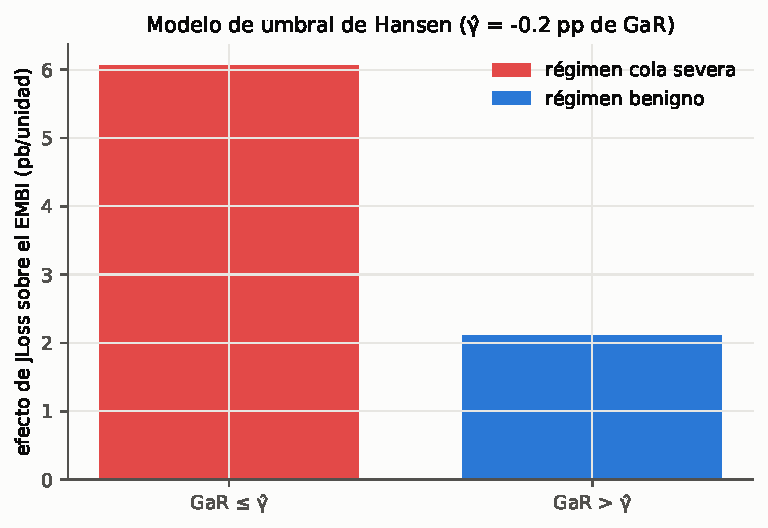
\includegraphics[width=0.55\textwidth]{fig_umbral.pdf}
\end{center}
\footnotesize Régimen de cola severa ($\GaR\le\hat\gamma=-0{,}18$ pp): efecto de $\JLoss$ sobre el EMBI $=+6{,}1$ pb/unidad. Régimen benigno: $+2{,}1$ pb. $LR=28{,}5$. El efecto es \textbf{casi tres veces mayor} cuando el crecimiento ya está en su cola izquierda.
\end{frame}

\begin{frame}{Identificación causal: qué se puede afirmar}
\begin{itemize}
\item \textbf{Proyecciones locales} (H1): respaldo dinámico directo, $+4{,}6$ pb ($t=2{,}9$).
\item \textbf{Variables instrumentales} (\textit{shift-share}): primera etapa aceptable ($F\approx11$) pero 2ª etapa no significativa; un segundo instrumento da signo opuesto; Sargan rechaza con los tres instrumentos probados.
\item \textbf{Regresores generados}: bootstrap de bloques por país (B=500, NLHPC) --- el error estándar crece apenas 2--15\%, ningún $p$-valor cambia de categoría.
\item \textbf{Wild cluster bootstrap} (13 \textit{clusters}): confirma la dimensión transversal ($p=0{,}015$ núcleo); la temporal queda marginal.
\end{itemize}
\vspace{6pt}
\begin{alertblock}{Honestidad estadística}
La identificación causal del canal de \emph{nivel} \textbf{no está cerrada} por variables instrumentales sobre esta muestra. La evidencia de H1 descansa en MCO con efectos fijos y proyecciones locales.
\end{alertblock}
\end{frame}

\section{Discusión y conclusiones}

\begin{frame}{Interpretación económica}
\begin{itemize}
\item El multiplicador de \textit{doom loop} se traslada al \textbf{precio} de la deuda soberana cuando el mercado espera que el pasivo contingente bancario recaiga sobre un soberano \textbf{no respaldado}.
\item El tenedor marginal que reprecia ese pasivo es un \textbf{inversor de cartera extranjero} --- no un banco o fondo de pensiones doméstico que mantiene la deuda a vencimiento.
\item Por eso la complementariedad:
  \begin{itemize}
  \item se \textbf{apaga} en economías de deuda local profunda (Polonia, India);
  \item se \textbf{apaga} bajo respaldo oficial masivo (\textit{Backstop});
  \item \textbf{sobrevive} en estrés sin respaldo (\textit{EMstress}).
  \end{itemize}
\end{itemize}
\vspace{8pt}
\centering
\textit{Es una propiedad de a quién y en qué régimen se le fija el precio a la deuda soberana --- no una regularidad universal de los mercados emergentes.}
\end{frame}

\begin{frame}{Conclusión}
Esta tesis retoma y precisa, con un panel más del triple de la muestra piloto y una batería de identificación mucho más exigente, la hipótesis con la que se aprobó su tema:
\vspace{4pt}
\begin{itemize}
\item Los canales de \textbf{nivel} (H1, H2) se sostienen con solidez.
\item La \textbf{complementariedad} (H3) es del signo predicho, pero \textbf{condicional}: no es un rasgo uniforme de todas las economías emergentes ni de todos los regímenes.
\item Un \textbf{test de falsación directo} (Backstop/EMstress) sostiene el mecanismo sin recurrir a excluir observaciones.
\end{itemize}
\vspace{8pt}
\begin{block}{El aporte}
No un coeficiente robusto a toda prueba --- la delimitación precisa de \emph{dónde} y \emph{cuándo} la complementariedad fragilidad--crecimiento aparece en los precios soberanos.
\end{block}
\end{frame}

\begin{frame}{Agenda futura}
\begin{itemize}
\item \textbf{Ampliar el grupo de contraste} de la heterogeneidad (hoy solo Polonia e India) y construir un moderador continuo de participación extranjera en la deuda.
\item \textbf{Ampliar el corte transversal} de $\JLoss$: Argentina, Egipto y Rusia solo les falta $\GaR$ o EMBI.
\item \textbf{Instrumentos adicionales} para el canal de nivel (choques de política monetaria identificados).
\item \textit{Pregunta abierta, no hallazgo:} ¿la concentración bancaria amplifica la complementariedad? No identificada con ninguno de 3 proxies de HHI --- el panel actual no tiene potencia estadística para dirimirlo.
\end{itemize}
\end{frame}

\section{Referencias}

\begin{frame}[allowframebreaks]{Referencias principales}
\footnotesize
\begin{itemize}
\item Chari, A., Garcés, F., Martínez, J. F., \& Valenzuela, P. (2024). Sovereign Credit Spreads, Banking Fragility, and Global Factors. \textit{Journal of Financial Stability}, 72, 101235.
\item Farhi, E., \& Tirole, J. (2018). Deadly Embrace: Sovereign and Financial Balance Sheets Doom Loops. \textit{Review of Economic Studies}, 85(3), 1781--1823.
\item Adrian, T., Boyarchenko, N., \& Giannone, D. (2019). Vulnerable Growth. \textit{American Economic Review}, 109(4), 1263--1289.
\item Acharya, V., Drechsler, I., \& Schnabl, P. (2014). A Pyrrhic Victory? Bank Bailouts and Sovereign Credit Risk. \textit{Journal of Finance}, 69(6), 2689--2739.
\item Hansen, B. E. (1999, 2000). Threshold Effects in Non-Dynamic Panels / Sample Splitting and Threshold Estimation.
\item Driscoll, J. C., \& Kraay, A. C. (1998). Consistent Covariance Matrix Estimation with Spatially Dependent Panel Data.
\item Cameron, A. C., Gelbach, J. B., \& Miller, D. L. (2008). Bootstrap-Based Improvements for Inference with Clustered Errors.
\item Ossandon Busch, M. et al. (2022). Growth at Risk: Methodology and Applications in an Open-Source Platform (CEMLA).
\end{itemize}
\end{frame}

\begin{frame}
\centering
\Large \textbf{Gracias}
\vspace{10pt}

\normalsize Repositorio reproducible: \texttt{1\_Codigo/Panel/bbg/}\\
Números canónicos: \texttt{NUMEROS\_CANONICOS\_BBG.md}
\vspace{14pt}

\large Preguntas
\end{frame}

\end{document}
